\subsection{实验目的-熟悉 iptables 的表链操作}
熟悉 iptables 的表链操作.
%
\subsection{实验原理}
通过 iptables 命令对防火墙 iptables 的表链进行相关操作(因环境策略不
同,表链会有所不同),如查看、添加、删除、修改等等。
%
\subsection{实验环境}
操作系统: CentOS 6.5
%
\subsection{实验步骤}
\subsubsection{Iptables 链操作}
查看 CentOS 6.5 中防火墙 iptables 的表名(因环境策略不同,表会有所不
同)。
在终端输入命令
\begin{minted}[bgcolor=bg,breaklines=true]{sh}
cat /proc/net/ip_tables_names
\end{minted}
若无结果,请查看是否开启服务。
可执行
\begin{minted}[bgcolor=bg,breaklines=true]{sh}
service iptables restart
\end{minted}
重启服务后再次执行,可以看到 iptables 包含 4 张表,
分别是 mangle、raw、filter 和 nat
(默认只有 filter 表,如果之前有对其他表进行过相关操作,才会有其他表)。
\begin{figure}[H]
  \begin{center}
    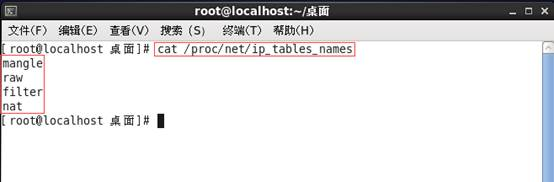
\includegraphics[width=0.40\textwidth]{2_5_1.jpeg}
  \end{center}
\end{figure}

在终端输入命令
\begin{minted}[bgcolor=bg,breaklines=true]{sh}
iptables -t filter -L
\end{minted}
查看表 filter 中的链及其链中的规则。
\mintinline{sh}{-t filter} 指定表 filter,也可不加,不加时默认表 filter。可知
表 filter 有 3 条链:
INPUT、FORWARD 和 OUTPUT,这 3 条链的默认规则都为 ACCEPT。
\begin{figure}[H]
  \begin{center}
    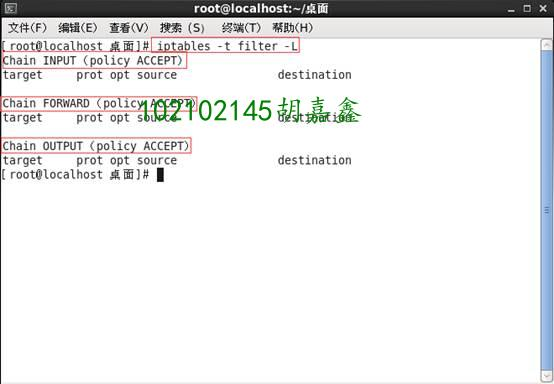
\includegraphics[width=0.40\textwidth]{2_5_2.jpeg}
  \end{center}
\end{figure}

若要查看某条链上的规则,在 \mintinline{sh}{-L} 参数后指明链名。
例如在终端输入命令
\begin{minted}[bgcolor=bg,breaklines=true]{sh}
iptables -L FORWARD
\end{minted}
查看表 filter 中链 FORWARD 上的规则。
\begin{figure}[H]
  \begin{center}
    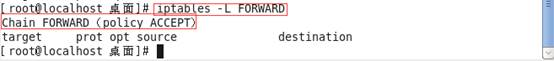
\includegraphics[width=0.40\textwidth]{2_5_3.jpeg}
  \end{center}
\end{figure}

在终端输入命令
\begin{minted}[bgcolor=bg,breaklines=true]{sh}
iptables -t nat –L
\end{minted}
查看表 nat 中的链及其链中的规则。
可知表 nat 有 3 条链:PREROUTING、POSTROUTING 和 OUTPUT,
这 3 条链的默认规则都为 ACCEPT。
\begin{figure}[H]
  \begin{center}
    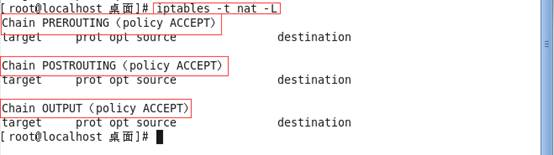
\includegraphics[width=0.40\textwidth]{2_5_4.jpeg}
  \end{center}
\end{figure}

在终端输入命令
\begin{minted}[bgcolor=bg,breaklines=true]{sh}
iptables -t mangle –L
\end{minted}
查看表 mangle 中的链及其链中的规则。
可知表 nat 有 5 条链:PREROUTING、INPUT、FORWARD、OUTPUT 和 POSTROUTING,
这 5 条链的默认规则都为 ACCEPT。
\begin{figure}[H]
  \begin{center}
    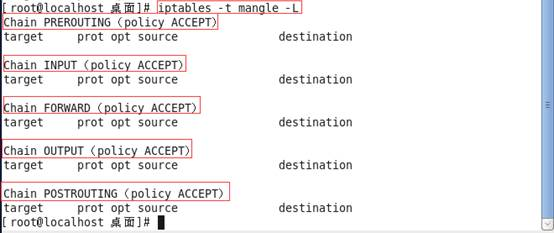
\includegraphics[width=0.40\textwidth]{2_5_5.jpeg}
  \end{center}
\end{figure}

在终端输入命令
\begin{minted}[bgcolor=bg,breaklines=true]{sh}
iptables -t raw –L
\end{minted}
查看表 nat 中的链及其链中的规则。
可知表 raw 有 2 条链:PREROUTING 和 OUTPUT,
这 2 条链的默认规则都为 ACCEPT。
\begin{figure}[H]
  \begin{center}
    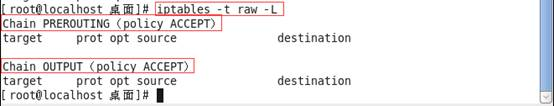
\includegraphics[width=0.40\textwidth]{2_5_6.jpeg}
  \end{center}
\end{figure}

在终端输入命令
\begin{minted}[bgcolor=bg,breaklines=true]{sh}
cat /etc/sysconfig/iptables
\end{minted}
(因环境策略不同,表中链及链中规则会有所不同),
查看防火墙配置文件,可以查看到 iptables 所有表中的链及其链中规则
(默认只有 filter 表,如果之前有对其他表进行过相关操作,才会有其他表)。
\begin{figure}[H]
  \begin{center}
    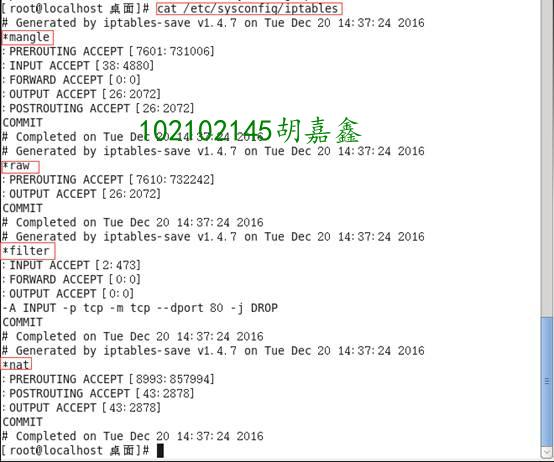
\includegraphics[width=0.40\textwidth]{2_5_7.jpeg}
  \end{center}
\end{figure}

这 4 张表 5 条链中的规则 target 为目标;prot 为协议;opt 为 option,
选项;source 为源地址,destination 为目的地址。在终端输入命令
\begin{minted}[bgcolor=bg,breaklines=true]{sh}
cat /proc/net/ip_tables_targets
\end{minted}
查看 iptables 中的 targets。
\begin{figure}[H]
  \begin{center}
    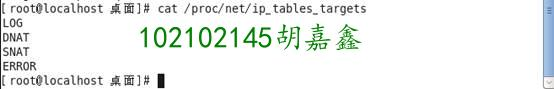
\includegraphics[width=0.40\textwidth]{2_5_8.jpeg}
  \end{center}
\end{figure}

在终端输入命令
\begin{minted}[bgcolor=bg,breaklines=true]{sh}
iptables -N simpleware1
\end{minted}
在表 filter 中添加一条名为 simpleware1 的新链。
这里没有使用 \mintinline{sh}{-t} 指定表,
默认是 filter 表,还可用 \mintinline{sh}{-t nat/mangle/raw}
在指定的表中添加新的链。再使用
\begin{minted}[bgcolor=bg,breaklines=true]{sh}
iptables -L
\end{minted}
进行查看。
\begin{figure}[H]
  \begin{center}
    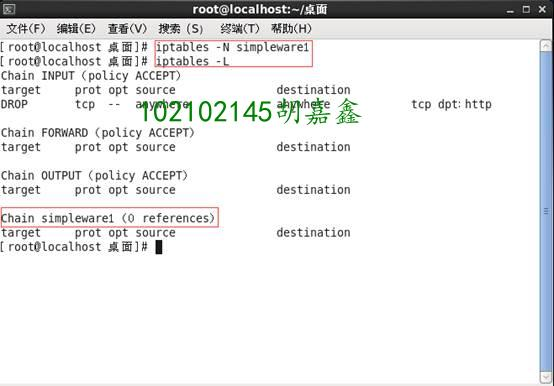
\includegraphics[width=0.40\textwidth]{2_5_9.jpeg}
  \end{center}
\end{figure}

使用上一步的方法继续在表 filter 中添加两条新链
simpleware2 和 simpleware3。
\begin{figure}[H]
  \begin{center}
    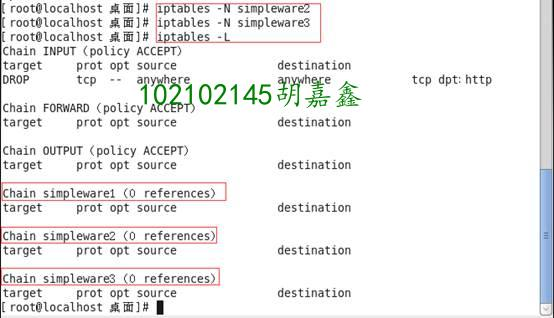
\includegraphics[width=0.40\textwidth]{2_5_10.jpeg}
  \end{center}
\end{figure}

若想删除某条自定义的链,使用 \mintinline{sh}{-X} 参数。
在终端输入命令
\begin{minted}[bgcolor=bg,breaklines=true]{sh}
iptables -X simpleware1
\end{minted}
删除表 filter 中自定义的链 simpleware1。
\begin{figure}[H]
  \begin{center}
    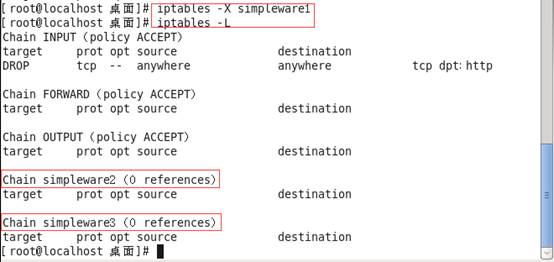
\includegraphics[width=0.40\textwidth]{2_5_11.jpeg}
  \end{center}
\end{figure}

在终端输入命令
\begin{minted}[bgcolor=bg,breaklines=true]{sh}
iptables -X
\end{minted}
直接删除表 filter 中所有自定义的链。
\begin{figure}[H]
  \begin{center}
    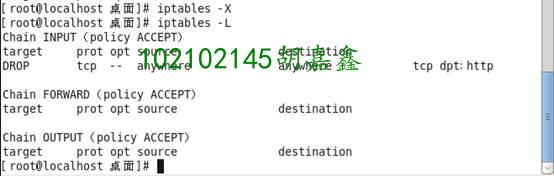
\includegraphics[width=0.40\textwidth]{2_5_12.jpeg}
  \end{center}
\end{figure}

可以使用 \mintinline{sh}{-P} 参数修改某条链的默认规则。
例如在终端输入命令
\begin{minted}[bgcolor=bg,breaklines=true]{sh}
iptables -P INPUT DROP
\end{minted}
将表 filter 中的链 INPUT 的默认规则改为 DROP。
\begin{figure}[H]
  \begin{center}
    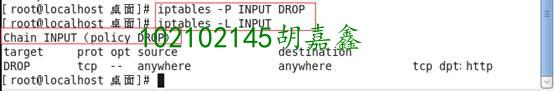
\includegraphics[width=0.40\textwidth]{2_5_13.jpeg}
  \end{center}
\end{figure}

在终端输入如下命令,分别在filter表的3条链上添加一条防火墙规则。
\begin{figure}[H]
  \begin{center}
    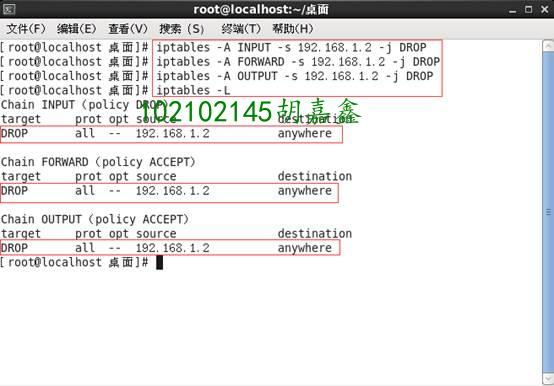
\includegraphics[width=0.40\textwidth]{2_5_14.jpeg}
  \end{center}
\end{figure}

在终端输入命令
\begin{minted}[bgcolor=bg,breaklines=true]{sh}
iptables -F INPUT
\end{minted}
清空 filter 表中 INPUT 链上的所有规则。
\begin{figure}[H]
  \begin{center}
    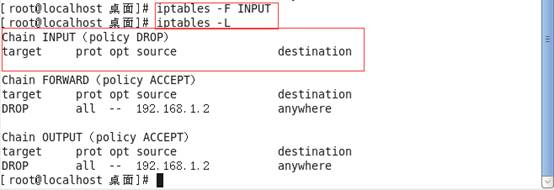
\includegraphics[width=0.40\textwidth]{2_5_15.jpeg}
  \end{center}
\end{figure}

在终端输入命令
\begin{minted}[bgcolor=bg,breaklines=true]{sh}
iptables -F
\end{minted}
不指明链名时,删除表 filter 中所有链上的规则。
\begin{figure}[H]
  \begin{center}
    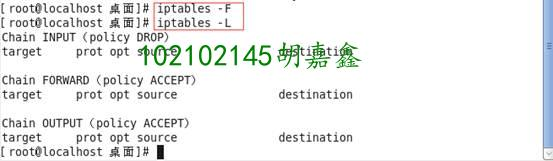
\includegraphics[width=0.40\textwidth]{2_5_16.jpeg}
  \end{center}
\end{figure}
